\subsection{Isomorphisms, Automorphisms, and the Orbit-Stabilizer Theorem}
Now, time for something completely different. Consider the structures
\begin{itemize}
\item $A$: $U^A=[3]$, $L^A=\{\op{1}{2},\op{1}{3}\}$, and
\item $B$: $U^B=[3]$, $L^B=\{\op{2}{1},\op{2}{3}\}$.
\end{itemize}
$A$ and $B$ look very similar. We can bring out their similarity by considering the the function $f:[3]\mapsto[3]$ with $f(1)=2$, $f(2)=1$, and $f(3)=3$. The function $f$ is a bijection and is edge-preserving, that is, for every $i,j\in[3]$, $\op{i}{j}\in L^A$ if and only if $\op{f(i)}{f(j)}\in L^B$. We say $f$ is an \emph{isomorphism} of $A$ onto $B$, and that $A$ and $B$ are \emph{isomorphic} (written $A\cong B$). These notions are so important that we pause to enshrine them in a definition.
\begin{definition}
A function $h$ is an \emph{isomorphism} from $A$ onto $B$ if and only if $h$ is a bijection from $U^A$ onto $U^B$ such that for all $a,b\in U^A$, $\op{a}{b}\in L^A$ if and only if $\op{h(a)}{h(b)}\in L^B$.

$A$ \emph{is isomorphic to} $B$ ($A\cong B$) if and only if there is an isomorphism $h$ from $A$ onto $B$.
\end{definition}
\begin{aside}
    Intuitively speaking, an isomorphism is a \emph{relabelling map}. The idea is that two structures are isomorphic if they ``look the same'' up to their nodes' names being ``relabelled''. In the example above, we ``relabelled'' $1$ as $2$ and $2$ as $1$. 
\end{aside}

Consider again the structure $A$ described above, but now consider the function $g$ with $g(1)=1$, $g(2)=3$, and $g(3)=2$. The function $g$ is an \emph{automorphism} of $A$, that is, an isomorphism of $A$ onto itself. Again, a definition is in order.
\begin{definition}
A function $h$ is an \emph{automorphism} of $A$  if and only if $h$ is an isomorphism of $A$ onto $A$. $\aut{A}=\{h\mid h\mbox{ is an automorphism of }A\}$.
\end{definition}

\begin{aside}
    An automorphism is an isomorphism (eg, a relabelling map) which leaves the edge-set unchanged (and hence leaves the whole structure unchanged). $h$ is an automorphism because the edges have exactly the same labels after the mapping. $f$ is not an automorphism, because the edges do not have the same labels after the mapping. 
\end{aside}

Note that if $A\cong B$, then for every schema $S$, $A\models S$ if and only if $B\models S$. Indeed, any theory which can reasonably call itself a Logic cannot distinguish isomorphic structures. 

\subsection*{The image of a structure}
Let's continue to consider the structure $A$. We have the following list of all the bijections of $[3]$ onto $[3]$.
\[
\begin{array}{|c|c|c|c|}
\hline
 &1&2&3\\
\hline
f_1&1&2&3\\
\hline
f_2&2&1&3\\
\hline
f_3&3&2&1\\
\hline
f_4&1&3&2\\
\hline
f_5&2&3&1\\
\hline
f_6&3&1&2\\
\hline

\end{array}
\]
We'll call this set of bijections $\symn{3}$ (more on this notation below). We define the \emph{image of a structure} as follows.

\begin{definition}
If $A$ is a graph with edge relation $L$ and $h$ a function, then the image of $A$ under $h$ is defined by
\[
    U^{h[A]} := U^A, L^{h[A]}=\{\op{h(i)}{h(j)}\mid\op{i}{j}\in L^A\}
\]
\end{definition}

It follows immediately that for any $C$ with $U^C = [3]$ and $h \in \symn{S}$, $h$ is an isomorphism from $C$ onto $h[C]$. 
With respect to the examples $A$ and $B$ above, we see that $B=f_2[A]$ and that $\aut{A}=\{f_1,f_4\}$. We also noted that $f_5[A]=B$ and that $f_3[A]=f_6[A]$ is a third isomorphic copy of $A$ distinct from both $A$ and $B$. That is, there are three labeled structures with universe $[3]$ that are isomorphic to $A$ - their respective automorphism classes are $\{f_1, f_4\}, \{f_2, f_5\}$, and $\{f_3, f_6\}$. 

\begin{center}
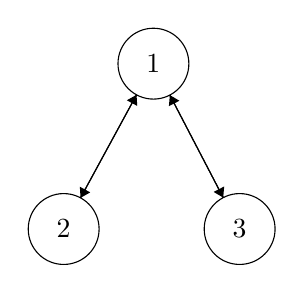
\begin{tikzpicture}[scale=0.15]
\tikzstyle{every node}+=[inner sep=0pt]
\draw [black] (38.9,-25.5) circle (3);
\draw (38.9,-25.5) node {$1$};
\draw [black] (31.3,-39.5) circle (3);
\draw (31.3,-39.5) node {$2$};
\draw [black] (46.2,-39.5) circle (3);
\draw (46.2,-39.5) node {$3$};
\draw [black] (37.47,-28.14) -- (32.73,-36.86);
\fill [black] (32.73,-36.86) -- (33.55,-36.4) -- (32.67,-35.92);
\draw [black] (32.73,-36.86) -- (37.47,-28.14);
\fill [black] (37.47,-28.14) -- (36.65,-28.6) -- (37.53,-29.08);
\draw [black] (40.29,-28.16) -- (44.81,-36.84);
\fill [black] (44.81,-36.84) -- (44.89,-35.9) -- (44,-36.36);
\draw [black] (44.81,-36.84) -- (40.29,-28.16);
\fill [black] (40.29,-28.16) -- (40.21,-29.1) -- (41.1,-28.64);
\end{tikzpicture}


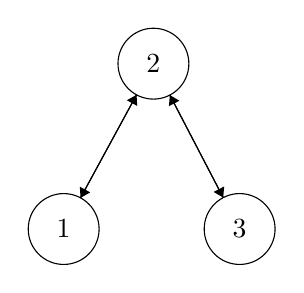
\begin{tikzpicture}[scale=0.15]
\tikzstyle{every node}+=[inner sep=0pt]
\draw [black] (38.9,-25.5) circle (3);
\draw (38.9,-25.5) node {$2$};
\draw [black] (31.3,-39.5) circle (3);
\draw (31.3,-39.5) node {$1$};
\draw [black] (46.2,-39.5) circle (3);
\draw (46.2,-39.5) node {$3$};
\draw [black] (37.47,-28.14) -- (32.73,-36.86);
\fill [black] (32.73,-36.86) -- (33.55,-36.4) -- (32.67,-35.92);
\draw [black] (32.73,-36.86) -- (37.47,-28.14);
\fill [black] (37.47,-28.14) -- (36.65,-28.6) -- (37.53,-29.08);
\draw [black] (40.29,-28.16) -- (44.81,-36.84);
\fill [black] (44.81,-36.84) -- (44.89,-35.9) -- (44,-36.36);
\draw [black] (44.81,-36.84) -- (40.29,-28.16);
\fill [black] (40.29,-28.16) -- (40.21,-29.1) -- (41.1,-28.64);
\end{tikzpicture}


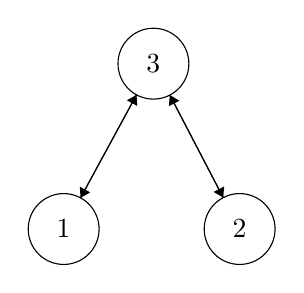
\begin{tikzpicture}[scale=0.15]
\tikzstyle{every node}+=[inner sep=0pt]
\draw [black] (38.9,-25.5) circle (3);
\draw (38.9,-25.5) node {$3$};
\draw [black] (31.3,-39.5) circle (3);
\draw (31.3,-39.5) node {$1$};
\draw [black] (46.2,-39.5) circle (3);
\draw (46.2,-39.5) node {$2$};
\draw [black] (37.47,-28.14) -- (32.73,-36.86);
\fill [black] (32.73,-36.86) -- (33.55,-36.4) -- (32.67,-35.92);
\draw [black] (32.73,-36.86) -- (37.47,-28.14);
\fill [black] (37.47,-28.14) -- (36.65,-28.6) -- (37.53,-29.08);
\draw [black] (40.29,-28.16) -- (44.81,-36.84);
\fill [black] (44.81,-36.84) -- (44.89,-35.9) -- (44,-36.36);
\draw [black] (44.81,-36.84) -- (40.29,-28.16);
\fill [black] (40.29,-28.16) -- (40.21,-29.1) -- (41.1,-28.64);
\end{tikzpicture}
\end{center}


This suggests the following marvelous identity, which we will shortly explore:
\begin{equation}\label{ose-eq}
\card{\symn{3}}=\card{\aut{A}}\cdot (\mbox{the number of labeled copies of }A).
\end{equation}

\subsection*{The Orbit-Stabilizer Theorem}

\begin{definition}
For every positive integer $k$ we write $[k]$ for $\{1,\ldots,k\}$
\end{definition}

\begin{definition}
For every positive integer $k$ we write $\symn{k}$ for the set of bijections from $[k]$ onto $[k]$ (also called the \emph{permutation group on} or the \emph{symmetric group on} $[k]$).
\end{definition}

The names \emph{permutation group} or \emph{symmetric group} emphasize the agebraic nature of \symn{k}. Indeed, we can think of \symn{k}\ as an algebra with a binary operation $\circ$, a unary operation $^{-1}$, and a distinguished element $e$, where, for permutations $f,g\in\symn{k}$, $f\circ g$ is the permutation resulting from the composition of $f$ and $g$, that is, $f\circ g =h$ if and only if for every $i\in [k]$, $h(i) = f(g(i))$; $f^{-1}$ is the permutation which is the inverse of $f$; and $e$ stands for the identity function on $[k]$. With these understandings, you can verify that \symn{k}\ is a group\footnote{These criteria (associativity, identity, inverse, closure) are the axioms for a \emph{group}, which is a fundamental and widely applicable concept in algebra. Group Theory, the part of mathematics which studies groups, is a hugely influential and interesting field. MATH 370 is Penn's introductory group theory course. }: 

\begin{itemize}
\item   
$\circ$ is an associative operation, that is, $(f\circ g)\circ h= f\circ (g\circ h)$, for all $f,g\in\symn{k}$;
\item
 $e$ is an identity with respect to $\circ$, that is, $e\circ f = f\circ e = f$, for all $f\in\symn{k}$; and 
 \item
 $f\circ f^{-1} = f^{-1}\circ f = e$, for all $f\in\symn{k}$.
 \item Permutations are closed under $\circ$, eg $f \circ g$ is a permutation for all $f, g \in \symn{k}$. 
\end{itemize} 

\begin{aside}
Prove that each of these criteria hold. 
\end{aside}

\begin{definition}
We write \sgraphn{k}\ for the set of simple graphs $A$ with $U^A = [k]$.
\end{definition}

\begin{definition}
For each $f\in\symn{k}$ and $A\in\sgraphn{k}$, we define $f[A]$ (called the \emph{image of the graph $A$ under $f$}) to be the graph with universe $[k]$ and edge-set
\[
    L^{f[A]} := \{\op{f(i)}{f(j)} \mid \op{i}{j} \in L^A\}
\]
Note that $f$ is an isomorphism of $A$ onto $f[A]$.
\end{definition}

The above definition is example of a \emph{group action} - the group \symn{k} \emph{acts on} the set \sgraphn{k}\ via the assignment of $f[A]$ to $A$. 

\begin{aside}
    Just as with groups, group actions are axiomatized by a few simple axioms. To verify that this is indeed a group action, show that for all $A\in\sgraphn{k}$ and $f,g\in\symn{k}$ the following properties hold:
    \begin{itemize}
    \item
    $(f\circ g)[A]=f[g[A]]$, and 
    \item
    $e[A]=A$.
    \end{itemize}    
\end{aside}


Recall that \aut{A}\ is the set of automorphisms of $A$. In the current context, for $A\in \sgraphn{k}$, \aut{A}\ is often called the \emph{stabilizer} of $A$, since $f\in\aut{A}$ if and only if $f[A] =A$. 

\begin{definition}
The \emph{orbit of} $A$  under the action of \symn{k}\ (written $\orb{A}{\symn{k}}$) is $\{h[A]\mid h\in\symn{k}\}$. 

In other words, the orbit of $A$ under \symn{k} is the maximal set of pairwise non-automorphic graphs which can be obtained from $A$ by actions in \symn{k}. 
\end{definition}

The following result is a special case of the \emph{Orbit-Stabilizer Theorem}.
\begin{theorem}\label{orb-stab-thm}
For all $A\in\sgraphn{n}$,
\[
\card{\symn{n}}=\card{\orb{A}{\symn{n}}}\cdot\card{\aut{A}}.
\]
\end{theorem}

\emph{Proof}:
Let $A\in\sgraphn{k}$. We define an equivalence relation $\sim$ on $\symn{k}$: for all $f,g\in\symn{k}$, $f\sim g$ if and only if $(f^{-1}\circ g)\in\aut{A}$. 

\begin{aside}
    Verify that $\sim$ is an equivalence relation, for example, it is reflexive (ie $f\sim f$), because $f^{-1}\circ f = e$ and $e\in \aut{A}$. Continue and show $\sim$ is symmetric and transitive.
\end{aside}

To establish the theorem, we prove two lemmata. 

We establish the following two claims about $\sim$ from which the Theorem follows immediately.
\begin{enumerate}
\item
each equivalence class of $\sim$ has size $\card{\aut{A}}$, and
\item
the number of equivalence classes of $\sim$ is $\card{\orb{A}{\symn{k}}}$.
\end{enumerate}
\emph{Ad} claim 1: Fix $f\in\symn{k}$. For each $h\in\aut{A}$ there is a unique $g\in\symn{k}$ such that $f^{-1}\circ g = h$. It follows at once that there is a bijection between $\{g\mid f\sim g\}$ and \aut{A}.

\begin{aside}
    Use the group axioms to first prove that inverses in a group are unique (eg for any $f$ in a group, there is a unique element $f^{-1}$ such that $f \circ f^{-1} = e = f^{-1} \circ f$, where $e$ is the identity element).

    Using that fact, verify that for each fixed $f, h \in \symn{k}$, the $g \in \symn{k}$ such that $f^{-1}\circ g = h$ is indeed unique. 
\end{aside}

\emph{Ad} claim 2: We show that for every $f,g\in\symn{k}$ $f[A]=g[A]$ if and only if $f\sim g$. We prove each direction of the bi-conditional. 

First, suppose suppose $f\sim g$. Then 
$f^{-1}\circ g \in \aut{A}$. It follows that $(f^{-1}\circ g)[A] = A$ and hence that $f[(f^{-1}\circ g)[A]] = f[A]$. So $(f\circ(f^{-1}\circ g))[A] = f[A]$, and then by associativity $((f\circ f^{-1})\circ g)[A] = f[A]$. As $f \circ f^{-1} = e$, we have $(e\circ g)[A] = f[A]$ from which it follows that $g[A]=f[A]$. 

In the other direction, suppose $f[A]=g[A]$. Then, $f^{-1}[f[A]]=f^{-1}[g[A]]$. Hence, $(f^{-1}\circ f)[A]=(f^{-1}\circ g)[A]$. Hence, $(f^{-1}\circ g)[A]=e[A]= A$. Hence, $f^{-1}\circ g\in \aut{A}$, that is, $f\sim g$. Thus, there is a bijection between the equivalence classes of $\sim$ and $\orb{A}{\symn{k}}$. \qed

We now have the explanation of identity (\ref{ose-eq}), since 
\[
\card{\orb{A}{\symn{k}}}=\mbox{the number of labeled copies of }A.
\]

In order to test out our new theorem\footnote{Look mom, I got a new Theorem for my birthday! I wanna play with it immediately!}, let's use it for some counting. Let $S$ be the conjunction of $\sg$ and $\oner$, that is, a graph $A$ satisfies $S$ if and only if $A$ is a 1-regular, simple graph. As we discussed earlier, every such finite graph $A$ has an even number, say $2n$, of nodes; moreover, if $A,B\models S$ and $\card{U^A}=\card{U^B}$, then $A$ is isomorphic to $B$. We will calculate the value of $\modn{S}{2n}$ in two ways - one way using the Orbit-Stabilizer Theorem, and the other directly. 

\subsubsection*{Via the Orbit-Stabilizer Theorem}
Let $A\in\modn{S}{2n}$. As we've just noted above, if $B\in\modn{S}{2n}$, then $A\cong B$. It follows at once that 
\begin{equation}\label{vos-eq}
\modn{S}{2n}=\orb{A}{\symn{2n}}.
\end{equation}
Let's calculate $\card{\aut{A}}$, since Theorem \ref{orb-stab-thm} will then allow us to calculate $\card{\modn{S}{2n}}$. Observe that $A$ consists of $n$ independent edges. Imagine them standing upright and lined up horizontally in some order. 

\begin{center}
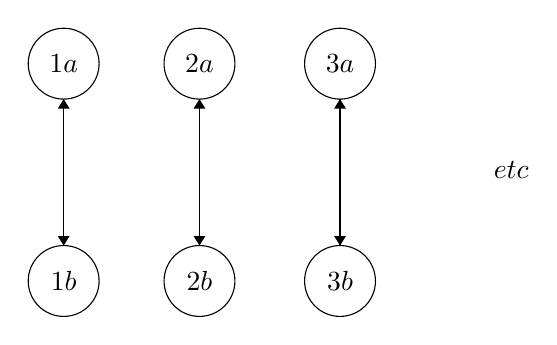
\begin{tikzpicture}[scale=0.15]
\tikzstyle{every node}+=[inner sep=0pt]
\draw [black] (22.2,-16) circle (3);
\draw (22.2,-16) node {$1a$};
\draw [black] (22.2,-34.4) circle (3);
\draw (22.2,-34.4) node {$1b$};
\draw [black] (33.7,-16) circle (3);
\draw (33.7,-16) node {$2a$};
\draw [black] (33.7,-34.4) circle (3);
\draw (33.7,-34.4) node {$2b$};
\draw [black] (45.6,-16) circle (3);
\draw (45.6,-16) node {$3a$};
\draw [black] (45.6,-34.4) circle (3);
\draw (45.6,-34.4) node {$3b$};
\draw (60.1,-25) node {$etc$};
\draw [black] (22.2,-19) -- (22.2,-31.4);
\fill [black] (22.2,-31.4) -- (22.7,-30.6) -- (21.7,-30.6);
\draw [black] (22.2,-31.4) -- (22.2,-19);
\fill [black] (22.2,-19) -- (21.7,-19.8) -- (22.7,-19.8);
\draw [black] (33.7,-19) -- (33.7,-31.4);
\fill [black] (33.7,-31.4) -- (34.2,-30.6) -- (33.2,-30.6);
\draw [black] (33.7,-31.4) -- (33.7,-19);
\fill [black] (33.7,-19) -- (33.2,-19.8) -- (34.2,-19.8);
\draw [black] (45.6,-19) -- (45.6,-31.4);
\fill [black] (45.6,-31.4) -- (46.1,-30.6) -- (45.1,-30.6);
\draw [black] (45.6,-31.4) -- (45.6,-19);
\fill [black] (45.6,-19) -- (45.1,-19.8) -- (46.1,-19.8);
\end{tikzpicture}
\end{center}

Now any permutation of the edges generates an automorphism of $A$. Moreover, in the process of permuting the edges, we have for each edge a choice whether to ``flip'' the edge or not. Since there are $n!$ permutations of the $n$ edges, and $2^n$ choices of which set of edges to flip, there are a total of $n!\cdot 2^n$ automorphisms of $A$. Hence, by Theorem \ref{orb-stab-thm} and equation (\ref{vos-eq}), 
 \[
 \card{\modn{S}{2n}}= (2n)!/n!\cdot 2^n.
 \]

\subsubsection*{Directly}
Here is a second direct method of calculating $\card{\modn{S}{2n}}$ which, thankfully, yields the same result\footnote{If it didn't, we'd have to agree that our new toy was broken, and would probably have a miserable rest of the day what with the inconvenience of having to return it and all.}. We construct a member $A$ of $\modn{S}{2n}$ as follows. We successively choose the $n$ independent edges that constitute $A$. So for the first edge, we have $\binom{2n}{2}$ choices of a pair of nodes between which to place an edge, and for the second edge, we have $\binom{2n-2}{2}$ choices, .... So the number of ways we can choose a sequence of $n$ independent edges is
\[
\binom{2n}{2}\cdot\binom{2n-2}{2}\cdots\binom{4}{2}\cdot\binom{2}{2}= \frac{(2n)!}{2^n}.
\]
Now any \emph{set} of $n$ edges chosen via this process will appear as the result of $n!$ such sequences of choices; thus, the total number of members of $\modn{S}{2n}$ we can construct is 
\[
\frac{(2n)!}{n!\cdot 2^n}.
\]